\begin{frame}{Perbandingan Kinerja Kumulatif: VQE vs Klasik (N=2)}
    \begin{figure}
        \centering
        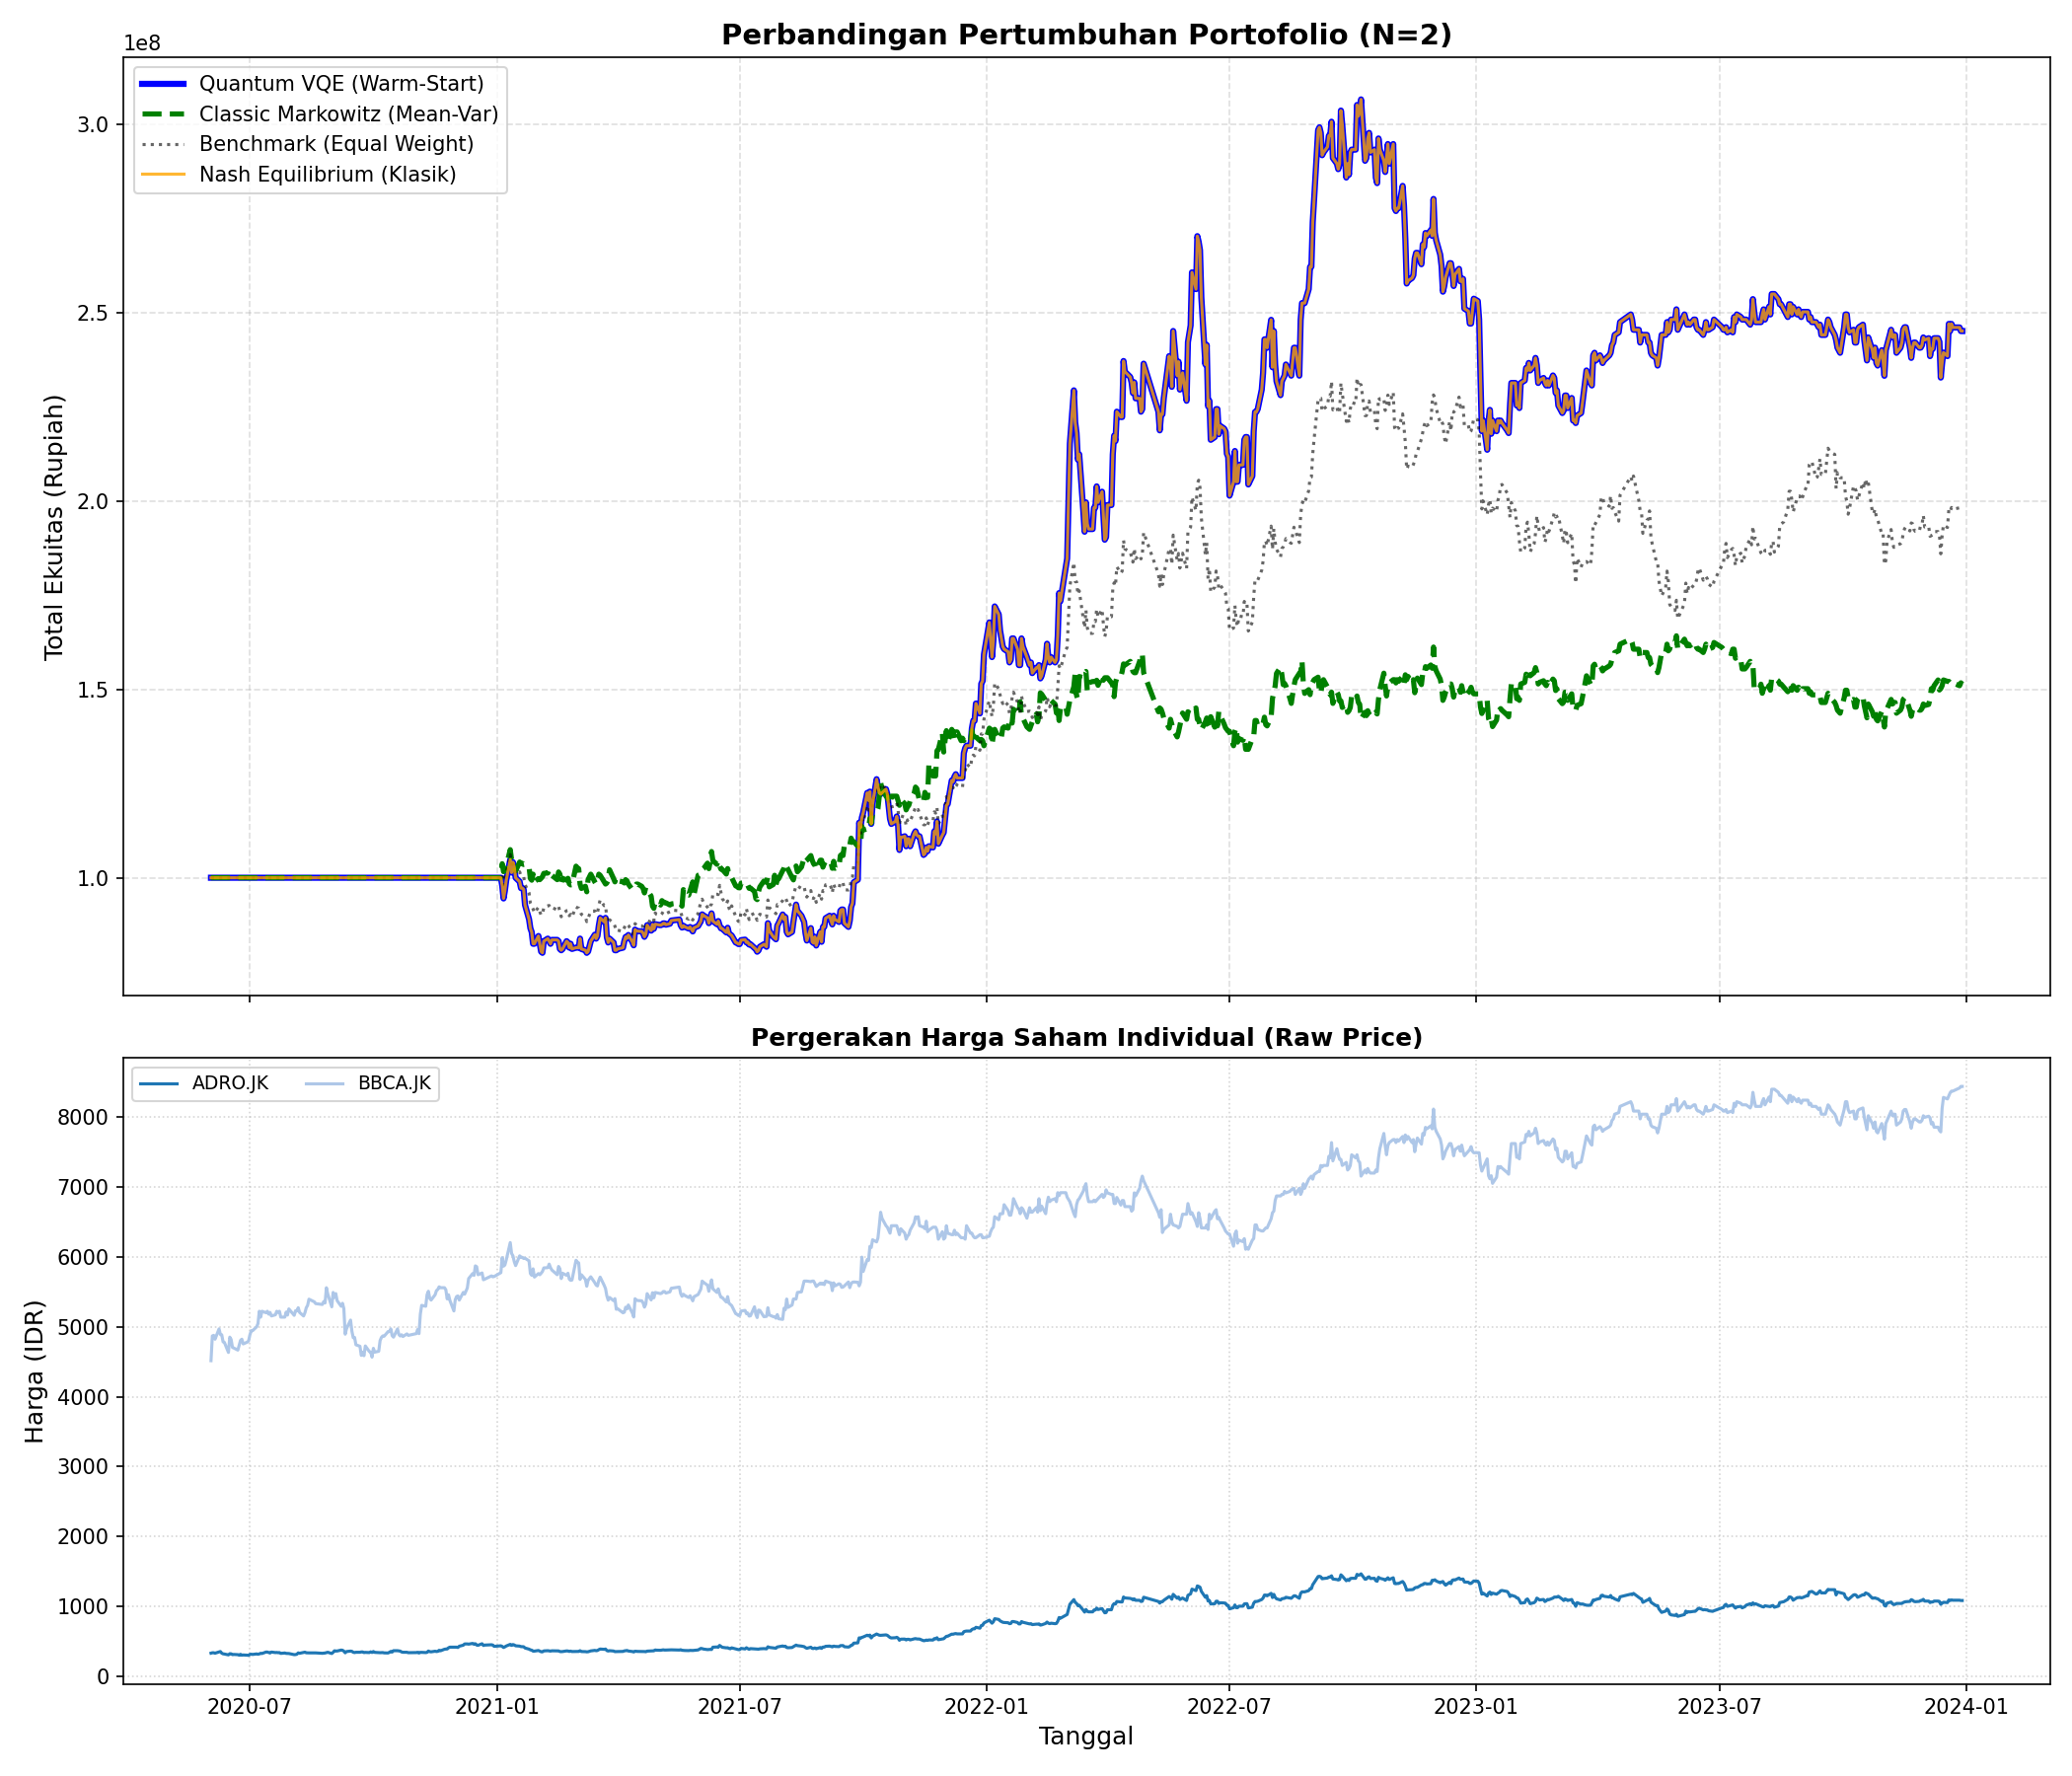
\includegraphics[width=0.8\textwidth]{../GTQuantumInvest/classic_compare/Grafik_Perbandingan/perbandingan_VQE_vs_Classic_N2.png}
        \caption{Perbandingan Pertumbuhan Modal Strategi VQE terhadap Tolok Ukur Klasik (N=2)}
    \end{figure}
\end{frame}

\begin{frame}{Perbandingan Alokasi Portofolio N=2 - 2021-01-04}
    \begin{figure}
        \centering
        \begin{subfigure}[b]{0.48\textwidth}
            \centering
            
\includegraphics[width=\textwidth]{../GTQuantumInvest/Hasil_N2_GT_5/Analisis_Window_N2/2021-01-04_window.png}
            \caption{Dengan \textit{Game Theory}}
        \end{subfigure}
        \hfill
        \begin{subfigure}[b]{0.48\textwidth}
            \centering
            
\includegraphics[width=\textwidth]{../GTQuantumInvest/Hasil_N2_NoGT_5/Analisis_Window_N2/2021-01-04_window.png}
            \caption{Tanpa \textit{Game Theory}}
        \end{subfigure}
        \caption{Jendela Waktu 2021-01-04}
    \end{figure}
\end{frame}

\begin{frame}{Perbandingan Sirkuit Kuantum N=2 - 2021-01-04}
    \begin{figure}
        \centering
        \begin{subfigure}[b]{0.48\textwidth}
            \centering
            
\includegraphics[width=\textwidth]{../GTQuantumInvest/Hasil_N2_GT_5/Analisis_Window_N2/2021-01-04_circuit.png}
            \caption{Sirkuit (GT)}
        \end{subfigure}
        \hfill
        \begin{subfigure}[b]{0.48\textwidth}
            \centering
            
\includegraphics[width=\textwidth]{../GTQuantumInvest/Hasil_N2_NoGT_5/Analisis_Window_N2/2021-01-04_circuit.png}
            \caption{Sirkuit (No-GT)}
        \end{subfigure}
        \caption{Perbandingan Rangkaian Kuantum - 2021-01-04}
    \end{figure}
\end{frame}

\begin{frame}{Perbandingan Alokasi Portofolio N=2 - 2021-02-02}
    \begin{figure}
        \centering
        \begin{subfigure}[b]{0.48\textwidth}
            \centering
            
\includegraphics[width=\textwidth]{../GTQuantumInvest/Hasil_N2_GT_5/Analisis_Window_N2/2021-02-02_window.png}
            \caption{Dengan \textit{Game Theory}}
        \end{subfigure}
        \hfill
        \begin{subfigure}[b]{0.48\textwidth}
            \centering
            
\includegraphics[width=\textwidth]{../GTQuantumInvest/Hasil_N2_NoGT_5/Analisis_Window_N2/2021-02-02_window.png}
            \caption{Tanpa \textit{Game Theory}}
        \end{subfigure}
        \caption{Jendela Waktu 2021-02-02}
    \end{figure}
\end{frame}

\begin{frame}{Perbandingan Sirkuit Kuantum N=2 - 2021-02-02}
    \begin{figure}
        \centering
        \begin{subfigure}[b]{0.48\textwidth}
            \centering
            
\includegraphics[width=\textwidth]{../GTQuantumInvest/Hasil_N2_GT_5/Analisis_Window_N2/2021-02-02_circuit.png}
            \caption{Sirkuit (GT)}
        \end{subfigure}
        \hfill
        \begin{subfigure}[b]{0.48\textwidth}
            \centering
            
\includegraphics[width=\textwidth]{../GTQuantumInvest/Hasil_N2_NoGT_5/Analisis_Window_N2/2021-02-02_circuit.png}
            \caption{Sirkuit (No-GT)}
        \end{subfigure}
        \caption{Perbandingan Rangkaian Kuantum - 2021-02-02}
    \end{figure}
\end{frame}

\begin{frame}{Perbandingan Alokasi Portofolio N=2 - 2021-03-04}
    \begin{figure}
        \centering
        \begin{subfigure}[b]{0.48\textwidth}
            \centering
            
\includegraphics[width=\textwidth]{../GTQuantumInvest/Hasil_N2_GT_5/Analisis_Window_N2/2021-03-04_window.png}
            \caption{Dengan \textit{Game Theory}}
        \end{subfigure}
        \hfill
        \begin{subfigure}[b]{0.48\textwidth}
            \centering
            
\includegraphics[width=\textwidth]{../GTQuantumInvest/Hasil_N2_NoGT_5/Analisis_Window_N2/2021-03-04_window.png}
            \caption{Tanpa \textit{Game Theory}}
        \end{subfigure}
        \caption{Jendela Waktu 2021-03-04}
    \end{figure}
\end{frame}

\begin{frame}{Perbandingan Sirkuit Kuantum N=2 - 2021-03-04}
    \begin{figure}
        \centering
        \begin{subfigure}[b]{0.48\textwidth}
            \centering
            
\includegraphics[width=\textwidth]{../GTQuantumInvest/Hasil_N2_GT_5/Analisis_Window_N2/2021-03-04_circuit.png}
            \caption{Sirkuit (GT)}
        \end{subfigure}
        \hfill
        \begin{subfigure}[b]{0.48\textwidth}
            \centering
            
\includegraphics[width=\textwidth]{../GTQuantumInvest/Hasil_N2_NoGT_5/Analisis_Window_N2/2021-03-04_circuit.png}
            \caption{Sirkuit (No-GT)}
        \end{subfigure}
        \caption{Perbandingan Rangkaian Kuantum - 2021-03-04}
    \end{figure}
\end{frame}

\begin{frame}{Perbandingan Alokasi Portofolio N=2 - 2021-04-06}
    \begin{figure}
        \centering
        \begin{subfigure}[b]{0.48\textwidth}
            \centering
            
\includegraphics[width=\textwidth]{../GTQuantumInvest/Hasil_N2_GT_5/Analisis_Window_N2/2021-04-06_window.png}
            \caption{Dengan \textit{Game Theory}}
        \end{subfigure}
        \hfill
        \begin{subfigure}[b]{0.48\textwidth}
            \centering
            
\includegraphics[width=\textwidth]{../GTQuantumInvest/Hasil_N2_NoGT_5/Analisis_Window_N2/2021-04-06_window.png}
            \caption{Tanpa \textit{Game Theory}}
        \end{subfigure}
        \caption{Jendela Waktu 2021-04-06}
    \end{figure}
\end{frame}

\begin{frame}{Perbandingan Sirkuit Kuantum N=2 - 2021-04-06}
    \begin{figure}
        \centering
        \begin{subfigure}[b]{0.48\textwidth}
            \centering
            
\includegraphics[width=\textwidth]{../GTQuantumInvest/Hasil_N2_GT_5/Analisis_Window_N2/2021-04-06_circuit.png}
            \caption{Sirkuit (GT)}
        \end{subfigure}
        \hfill
        \begin{subfigure}[b]{0.48\textwidth}
            \centering
            
\includegraphics[width=\textwidth]{../GTQuantumInvest/Hasil_N2_NoGT_5/Analisis_Window_N2/2021-04-06_circuit.png}
            \caption{Sirkuit (No-GT)}
        \end{subfigure}
        \caption{Perbandingan Rangkaian Kuantum - 2021-04-06}
    \end{figure}
\end{frame}

\begin{frame}{Perbandingan Alokasi Portofolio N=2 - 2021-05-05}
    \begin{figure}
        \centering
        \begin{subfigure}[b]{0.48\textwidth}
            \centering
            
\includegraphics[width=\textwidth]{../GTQuantumInvest/Hasil_N2_GT_5/Analisis_Window_N2/2021-05-05_window.png}
            \caption{Dengan \textit{Game Theory}}
        \end{subfigure}
        \hfill
        \begin{subfigure}[b]{0.48\textwidth}
            \centering
            
\includegraphics[width=\textwidth]{../GTQuantumInvest/Hasil_N2_NoGT_5/Analisis_Window_N2/2021-05-05_window.png}
            \caption{Tanpa \textit{Game Theory}}
        \end{subfigure}
        \caption{Jendela Waktu 2021-05-05}
    \end{figure}
\end{frame}

\begin{frame}{Perbandingan Sirkuit Kuantum N=2 - 2021-05-05}
    \begin{figure}
        \centering
        \begin{subfigure}[b]{0.48\textwidth}
            \centering
            
\includegraphics[width=\textwidth]{../GTQuantumInvest/Hasil_N2_GT_5/Analisis_Window_N2/2021-05-05_circuit.png}
            \caption{Sirkuit (GT)}
        \end{subfigure}
        \hfill
        \begin{subfigure}[b]{0.48\textwidth}
            \centering
            
\includegraphics[width=\textwidth]{../GTQuantumInvest/Hasil_N2_NoGT_5/Analisis_Window_N2/2021-05-05_circuit.png}
            \caption{Sirkuit (No-GT)}
        \end{subfigure}
        \caption{Perbandingan Rangkaian Kuantum - 2021-05-05}
    \end{figure}
\end{frame}

\begin{frame}{Perbandingan Alokasi Portofolio N=2 - 2021-06-10}
    \begin{figure}
        \centering
        \begin{subfigure}[b]{0.48\textwidth}
            \centering
            
\includegraphics[width=\textwidth]{../GTQuantumInvest/Hasil_N2_GT_5/Analisis_Window_N2/2021-06-10_window.png}
            \caption{Dengan \textit{Game Theory}}
        \end{subfigure}
        \hfill
        \begin{subfigure}[b]{0.48\textwidth}
            \centering
            
\includegraphics[width=\textwidth]{../GTQuantumInvest/Hasil_N2_NoGT_5/Analisis_Window_N2/2021-06-10_window.png}
            \caption{Tanpa \textit{Game Theory}}
        \end{subfigure}
        \caption{Jendela Waktu 2021-06-10}
    \end{figure}
\end{frame}

\begin{frame}{Perbandingan Sirkuit Kuantum N=2 - 2021-06-10}
    \begin{figure}
        \centering
        \begin{subfigure}[b]{0.48\textwidth}
            \centering
            
\includegraphics[width=\textwidth]{../GTQuantumInvest/Hasil_N2_GT_5/Analisis_Window_N2/2021-06-10_circuit.png}
            \caption{Sirkuit (GT)}
        \end{subfigure}
        \hfill
        \begin{subfigure}[b]{0.48\textwidth}
            \centering
            
\includegraphics[width=\textwidth]{../GTQuantumInvest/Hasil_N2_NoGT_5/Analisis_Window_N2/2021-06-10_circuit.png}
            \caption{Sirkuit (No-GT)}
        \end{subfigure}
        \caption{Perbandingan Rangkaian Kuantum - 2021-06-10}
    \end{figure}
\end{frame}

\begin{frame}{Perbandingan Alokasi Portofolio N=2 - 2021-07-09}
    \begin{figure}
        \centering
        \begin{subfigure}[b]{0.48\textwidth}
            \centering
            
\includegraphics[width=\textwidth]{../GTQuantumInvest/Hasil_N2_GT_5/Analisis_Window_N2/2021-07-09_window.png}
            \caption{Dengan \textit{Game Theory}}
        \end{subfigure}
        \hfill
        \begin{subfigure}[b]{0.48\textwidth}
            \centering
            
\includegraphics[width=\textwidth]{../GTQuantumInvest/Hasil_N2_NoGT_5/Analisis_Window_N2/2021-07-09_window.png}
            \caption{Tanpa \textit{Game Theory}}
        \end{subfigure}
        \caption{Jendela Waktu 2021-07-09}
    \end{figure}
\end{frame}

\begin{frame}{Perbandingan Sirkuit Kuantum N=2 - 2021-07-09}
    \begin{figure}
        \centering
        \begin{subfigure}[b]{0.48\textwidth}
            \centering
            
\includegraphics[width=\textwidth]{../GTQuantumInvest/Hasil_N2_GT_5/Analisis_Window_N2/2021-07-09_circuit.png}
            \caption{Sirkuit (GT)}
        \end{subfigure}
        \hfill
        \begin{subfigure}[b]{0.48\textwidth}
            \centering
            
\includegraphics[width=\textwidth]{../GTQuantumInvest/Hasil_N2_NoGT_5/Analisis_Window_N2/2021-07-09_circuit.png}
            \caption{Sirkuit (No-GT)}
        \end{subfigure}
        \caption{Perbandingan Rangkaian Kuantum - 2021-07-09}
    \end{figure}
\end{frame}

\begin{frame}{Perbandingan Alokasi Portofolio N=2 - 2021-08-10}
    \begin{figure}
        \centering
        \begin{subfigure}[b]{0.48\textwidth}
            \centering
            
\includegraphics[width=\textwidth]{../GTQuantumInvest/Hasil_N2_GT_5/Analisis_Window_N2/2021-08-10_window.png}
            \caption{Dengan \textit{Game Theory}}
        \end{subfigure}
        \hfill
        \begin{subfigure}[b]{0.48\textwidth}
            \centering
            
\includegraphics[width=\textwidth]{../GTQuantumInvest/Hasil_N2_NoGT_5/Analisis_Window_N2/2021-08-10_window.png}
            \caption{Tanpa \textit{Game Theory}}
        \end{subfigure}
        \caption{Jendela Waktu 2021-08-10}
    \end{figure}
\end{frame}

\begin{frame}{Perbandingan Sirkuit Kuantum N=2 - 2021-08-10}
    \begin{figure}
        \centering
        \begin{subfigure}[b]{0.48\textwidth}
            \centering
            
\includegraphics[width=\textwidth]{../GTQuantumInvest/Hasil_N2_GT_5/Analisis_Window_N2/2021-08-10_circuit.png}
            \caption{Sirkuit (GT)}
        \end{subfigure}
        \hfill
        \begin{subfigure}[b]{0.48\textwidth}
            \centering
            
\includegraphics[width=\textwidth]{../GTQuantumInvest/Hasil_N2_NoGT_5/Analisis_Window_N2/2021-08-10_circuit.png}
            \caption{Sirkuit (No-GT)}
        \end{subfigure}
        \caption{Perbandingan Rangkaian Kuantum - 2021-08-10}
    \end{figure}
\end{frame}

\begin{frame}{Perbandingan Alokasi Portofolio N=2 - 2021-09-10}
    \begin{figure}
        \centering
        \begin{subfigure}[b]{0.48\textwidth}
            \centering
            
\includegraphics[width=\textwidth]{../GTQuantumInvest/Hasil_N2_GT_5/Analisis_Window_N2/2021-09-10_window.png}
            \caption{Dengan \textit{Game Theory}}
        \end{subfigure}
        \hfill
        \begin{subfigure}[b]{0.48\textwidth}
            \centering
            
\includegraphics[width=\textwidth]{../GTQuantumInvest/Hasil_N2_NoGT_5/Analisis_Window_N2/2021-09-10_window.png}
            \caption{Tanpa \textit{Game Theory}}
        \end{subfigure}
        \caption{Jendela Waktu 2021-09-10}
    \end{figure}
\end{frame}

\begin{frame}{Perbandingan Sirkuit Kuantum N=2 - 2021-09-10}
    \begin{figure}
        \centering
        \begin{subfigure}[b]{0.48\textwidth}
            \centering
            
\includegraphics[width=\textwidth]{../GTQuantumInvest/Hasil_N2_GT_5/Analisis_Window_N2/2021-09-10_circuit.png}
            \caption{Sirkuit (GT)}
        \end{subfigure}
        \hfill
        \begin{subfigure}[b]{0.48\textwidth}
            \centering
            
\includegraphics[width=\textwidth]{../GTQuantumInvest/Hasil_N2_NoGT_5/Analisis_Window_N2/2021-09-10_circuit.png}
            \caption{Sirkuit (No-GT)}
        \end{subfigure}
        \caption{Perbandingan Rangkaian Kuantum - 2021-09-10}
    \end{figure}
\end{frame}

\begin{frame}{Perbandingan Alokasi Portofolio N=2 - 2021-10-11}
    \begin{figure}
        \centering
        \begin{subfigure}[b]{0.48\textwidth}
            \centering
            
\includegraphics[width=\textwidth]{../GTQuantumInvest/Hasil_N2_GT_5/Analisis_Window_N2/2021-10-11_window.png}
            \caption{Dengan \textit{Game Theory}}
        \end{subfigure}
        \hfill
        \begin{subfigure}[b]{0.48\textwidth}
            \centering
            
\includegraphics[width=\textwidth]{../GTQuantumInvest/Hasil_N2_NoGT_5/Analisis_Window_N2/2021-10-11_window.png}
            \caption{Tanpa \textit{Game Theory}}
        \end{subfigure}
        \caption{Jendela Waktu 2021-10-11}
    \end{figure}
\end{frame}

\begin{frame}{Perbandingan Sirkuit Kuantum N=2 - 2021-10-11}
    \begin{figure}
        \centering
        \begin{subfigure}[b]{0.48\textwidth}
            \centering
            
\includegraphics[width=\textwidth]{../GTQuantumInvest/Hasil_N2_GT_5/Analisis_Window_N2/2021-10-11_circuit.png}
            \caption{Sirkuit (GT)}
        \end{subfigure}
        \hfill
        \begin{subfigure}[b]{0.48\textwidth}
            \centering
            
\includegraphics[width=\textwidth]{../GTQuantumInvest/Hasil_N2_NoGT_5/Analisis_Window_N2/2021-10-11_circuit.png}
            \caption{Sirkuit (No-GT)}
        \end{subfigure}
        \caption{Perbandingan Rangkaian Kuantum - 2021-10-11}
    \end{figure}
\end{frame}

\begin{frame}{Perbandingan Alokasi Portofolio N=2 - 2021-11-10}
    \begin{figure}
        \centering
        \begin{subfigure}[b]{0.48\textwidth}
            \centering
            
\includegraphics[width=\textwidth]{../GTQuantumInvest/Hasil_N2_GT_5/Analisis_Window_N2/2021-11-10_window.png}
            \caption{Dengan \textit{Game Theory}}
        \end{subfigure}
        \hfill
        \begin{subfigure}[b]{0.48\textwidth}
            \centering
            
\includegraphics[width=\textwidth]{../GTQuantumInvest/Hasil_N2_NoGT_5/Analisis_Window_N2/2021-11-10_window.png}
            \caption{Tanpa \textit{Game Theory}}
        \end{subfigure}
        \caption{Jendela Waktu 2021-11-10}
    \end{figure}
\end{frame}

\begin{frame}{Perbandingan Sirkuit Kuantum N=2 - 2021-11-10}
    \begin{figure}
        \centering
        \begin{subfigure}[b]{0.48\textwidth}
            \centering
            
\includegraphics[width=\textwidth]{../GTQuantumInvest/Hasil_N2_GT_5/Analisis_Window_N2/2021-11-10_circuit.png}
            \caption{Sirkuit (GT)}
        \end{subfigure}
        \hfill
        \begin{subfigure}[b]{0.48\textwidth}
            \centering
            
\includegraphics[width=\textwidth]{../GTQuantumInvest/Hasil_N2_NoGT_5/Analisis_Window_N2/2021-11-10_circuit.png}
            \caption{Sirkuit (No-GT)}
        \end{subfigure}
        \caption{Perbandingan Rangkaian Kuantum - 2021-11-10}
    \end{figure}
\end{frame}

\begin{frame}{Perbandingan Alokasi Portofolio N=2 - 2021-12-09}
    \begin{figure}
        \centering
        \begin{subfigure}[b]{0.48\textwidth}
            \centering
            
\includegraphics[width=\textwidth]{../GTQuantumInvest/Hasil_N2_GT_5/Analisis_Window_N2/2021-12-09_window.png}
            \caption{Dengan \textit{Game Theory}}
        \end{subfigure}
        \hfill
        \begin{subfigure}[b]{0.48\textwidth}
            \centering
            
\includegraphics[width=\textwidth]{../GTQuantumInvest/Hasil_N2_NoGT_5/Analisis_Window_N2/2021-12-09_window.png}
            \caption{Tanpa \textit{Game Theory}}
        \end{subfigure}
        \caption{Jendela Waktu 2021-12-09}
    \end{figure}
\end{frame}

\begin{frame}{Perbandingan Sirkuit Kuantum N=2 - 2021-12-09}
    \begin{figure}
        \centering
        \begin{subfigure}[b]{0.48\textwidth}
            \centering
            
\includegraphics[width=\textwidth]{../GTQuantumInvest/Hasil_N2_GT_5/Analisis_Window_N2/2021-12-09_circuit.png}
            \caption{Sirkuit (GT)}
        \end{subfigure}
        \hfill
        \begin{subfigure}[b]{0.48\textwidth}
            \centering
            
\includegraphics[width=\textwidth]{../GTQuantumInvest/Hasil_N2_NoGT_5/Analisis_Window_N2/2021-12-09_circuit.png}
            \caption{Sirkuit (No-GT)}
        \end{subfigure}
        \caption{Perbandingan Rangkaian Kuantum - 2021-12-09}
    \end{figure}
\end{frame}

\begin{frame}{Perbandingan Alokasi Portofolio N=2 - 2022-01-10}
    \begin{figure}
        \centering
        \begin{subfigure}[b]{0.48\textwidth}
            \centering
            
\includegraphics[width=\textwidth]{../GTQuantumInvest/Hasil_N2_GT_5/Analisis_Window_N2/2022-01-10_window.png}
            \caption{Dengan \textit{Game Theory}}
        \end{subfigure}
        \hfill
        \begin{subfigure}[b]{0.48\textwidth}
            \centering
            
\includegraphics[width=\textwidth]{../GTQuantumInvest/Hasil_N2_NoGT_5/Analisis_Window_N2/2022-01-10_window.png}
            \caption{Tanpa \textit{Game Theory}}
        \end{subfigure}
        \caption{Jendela Waktu 2022-01-10}
    \end{figure}
\end{frame}

\begin{frame}{Perbandingan Sirkuit Kuantum N=2 - 2022-01-10}
    \begin{figure}
        \centering
        \begin{subfigure}[b]{0.48\textwidth}
            \centering
            
\includegraphics[width=\textwidth]{../GTQuantumInvest/Hasil_N2_GT_5/Analisis_Window_N2/2022-01-10_circuit.png}
            \caption{Sirkuit (GT)}
        \end{subfigure}
        \hfill
        \begin{subfigure}[b]{0.48\textwidth}
            \centering
            
\includegraphics[width=\textwidth]{../GTQuantumInvest/Hasil_N2_NoGT_5/Analisis_Window_N2/2022-01-10_circuit.png}
            \caption{Sirkuit (No-GT)}
        \end{subfigure}
        \caption{Perbandingan Rangkaian Kuantum - 2022-01-10}
    \end{figure}
\end{frame}

\begin{frame}{Perbandingan Alokasi Portofolio N=2 - 2022-02-09}
    \begin{figure}
        \centering
        \begin{subfigure}[b]{0.48\textwidth}
            \centering
            
\includegraphics[width=\textwidth]{../GTQuantumInvest/Hasil_N2_GT_5/Analisis_Window_N2/2022-02-09_window.png}
            \caption{Dengan \textit{Game Theory}}
        \end{subfigure}
        \hfill
        \begin{subfigure}[b]{0.48\textwidth}
            \centering
            
\includegraphics[width=\textwidth]{../GTQuantumInvest/Hasil_N2_NoGT_5/Analisis_Window_N2/2022-02-09_window.png}
            \caption{Tanpa \textit{Game Theory}}
        \end{subfigure}
        \caption{Jendela Waktu 2022-02-09}
    \end{figure}
\end{frame}

\begin{frame}{Perbandingan Sirkuit Kuantum N=2 - 2022-02-09}
    \begin{figure}
        \centering
        \begin{subfigure}[b]{0.48\textwidth}
            \centering
            
\includegraphics[width=\textwidth]{../GTQuantumInvest/Hasil_N2_GT_5/Analisis_Window_N2/2022-02-09_circuit.png}
            \caption{Sirkuit (GT)}
        \end{subfigure}
        \hfill
        \begin{subfigure}[b]{0.48\textwidth}
            \centering
            
\includegraphics[width=\textwidth]{../GTQuantumInvest/Hasil_N2_NoGT_5/Analisis_Window_N2/2022-02-09_circuit.png}
            \caption{Sirkuit (No-GT)}
        \end{subfigure}
        \caption{Perbandingan Rangkaian Kuantum - 2022-02-09}
    \end{figure}
\end{frame}

\begin{frame}{Perbandingan Alokasi Portofolio N=2 - 2022-03-14}
    \begin{figure}
        \centering
        \begin{subfigure}[b]{0.48\textwidth}
            \centering
            
\includegraphics[width=\textwidth]{../GTQuantumInvest/Hasil_N2_GT_5/Analisis_Window_N2/2022-03-14_window.png}
            \caption{Dengan \textit{Game Theory}}
        \end{subfigure}
        \hfill
        \begin{subfigure}[b]{0.48\textwidth}
            \centering
            
\includegraphics[width=\textwidth]{../GTQuantumInvest/Hasil_N2_NoGT_5/Analisis_Window_N2/2022-03-14_window.png}
            \caption{Tanpa \textit{Game Theory}}
        \end{subfigure}
        \caption{Jendela Waktu 2022-03-14}
    \end{figure}
\end{frame}

\begin{frame}{Perbandingan Sirkuit Kuantum N=2 - 2022-03-14}
    \begin{figure}
        \centering
        \begin{subfigure}[b]{0.48\textwidth}
            \centering
            
\includegraphics[width=\textwidth]{../GTQuantumInvest/Hasil_N2_GT_5/Analisis_Window_N2/2022-03-14_circuit.png}
            \caption{Sirkuit (GT)}
        \end{subfigure}
        \hfill
        \begin{subfigure}[b]{0.48\textwidth}
            \centering
            
\includegraphics[width=\textwidth]{../GTQuantumInvest/Hasil_N2_NoGT_5/Analisis_Window_N2/2022-03-14_circuit.png}
            \caption{Sirkuit (No-GT)}
        \end{subfigure}
        \caption{Perbandingan Rangkaian Kuantum - 2022-03-14}
    \end{figure}
\end{frame}

\begin{frame}{Perbandingan Alokasi Portofolio N=2 - 2022-04-12}
    \begin{figure}
        \centering
        \begin{subfigure}[b]{0.48\textwidth}
            \centering
            
\includegraphics[width=\textwidth]{../GTQuantumInvest/Hasil_N2_GT_5/Analisis_Window_N2/2022-04-12_window.png}
            \caption{Dengan \textit{Game Theory}}
        \end{subfigure}
        \hfill
        \begin{subfigure}[b]{0.48\textwidth}
            \centering
            
\includegraphics[width=\textwidth]{../GTQuantumInvest/Hasil_N2_NoGT_5/Analisis_Window_N2/2022-04-12_window.png}
            \caption{Tanpa \textit{Game Theory}}
        \end{subfigure}
        \caption{Jendela Waktu 2022-04-12}
    \end{figure}
\end{frame}

\begin{frame}{Perbandingan Sirkuit Kuantum N=2 - 2022-04-12}
    \begin{figure}
        \centering
        \begin{subfigure}[b]{0.48\textwidth}
            \centering
            
\includegraphics[width=\textwidth]{../GTQuantumInvest/Hasil_N2_GT_5/Analisis_Window_N2/2022-04-12_circuit.png}
            \caption{Sirkuit (GT)}
        \end{subfigure}
        \hfill
        \begin{subfigure}[b]{0.48\textwidth}
            \centering
            
\includegraphics[width=\textwidth]{../GTQuantumInvest/Hasil_N2_NoGT_5/Analisis_Window_N2/2022-04-12_circuit.png}
            \caption{Sirkuit (No-GT)}
        \end{subfigure}
        \caption{Perbandingan Rangkaian Kuantum - 2022-04-12}
    \end{figure}
\end{frame}

\begin{frame}{Perbandingan Alokasi Portofolio N=2 - 2022-05-23}
    \begin{figure}
        \centering
        \begin{subfigure}[b]{0.48\textwidth}
            \centering
            
\includegraphics[width=\textwidth]{../GTQuantumInvest/Hasil_N2_GT_5/Analisis_Window_N2/2022-05-23_window.png}
            \caption{Dengan \textit{Game Theory}}
        \end{subfigure}
        \hfill
        \begin{subfigure}[b]{0.48\textwidth}
            \centering
            
\includegraphics[width=\textwidth]{../GTQuantumInvest/Hasil_N2_NoGT_5/Analisis_Window_N2/2022-05-23_window.png}
            \caption{Tanpa \textit{Game Theory}}
        \end{subfigure}
        \caption{Jendela Waktu 2022-05-23}
    \end{figure}
\end{frame}

\begin{frame}{Perbandingan Sirkuit Kuantum N=2 - 2022-05-23}
    \begin{figure}
        \centering
        \begin{subfigure}[b]{0.48\textwidth}
            \centering
            
\includegraphics[width=\textwidth]{../GTQuantumInvest/Hasil_N2_GT_5/Analisis_Window_N2/2022-05-23_circuit.png}
            \caption{Sirkuit (GT)}
        \end{subfigure}
        \hfill
        \begin{subfigure}[b]{0.48\textwidth}
            \centering
            
\includegraphics[width=\textwidth]{../GTQuantumInvest/Hasil_N2_NoGT_5/Analisis_Window_N2/2022-05-23_circuit.png}
            \caption{Sirkuit (No-GT)}
        \end{subfigure}
        \caption{Perbandingan Rangkaian Kuantum - 2022-05-23}
    \end{figure}
\end{frame}

\begin{frame}{Perbandingan Alokasi Portofolio N=2 - 2022-06-23}
    \begin{figure}
        \centering
        \begin{subfigure}[b]{0.48\textwidth}
            \centering
            
\includegraphics[width=\textwidth]{../GTQuantumInvest/Hasil_N2_GT_5/Analisis_Window_N2/2022-06-23_window.png}
            \caption{Dengan \textit{Game Theory}}
        \end{subfigure}
        \hfill
        \begin{subfigure}[b]{0.48\textwidth}
            \centering
            
\includegraphics[width=\textwidth]{../GTQuantumInvest/Hasil_N2_NoGT_5/Analisis_Window_N2/2022-06-23_window.png}
            \caption{Tanpa \textit{Game Theory}}
        \end{subfigure}
        \caption{Jendela Waktu 2022-06-23}
    \end{figure}
\end{frame}

\begin{frame}{Perbandingan Sirkuit Kuantum N=2 - 2022-06-23}
    \begin{figure}
        \centering
        \begin{subfigure}[b]{0.48\textwidth}
            \centering
            
\includegraphics[width=\textwidth]{../GTQuantumInvest/Hasil_N2_GT_5/Analisis_Window_N2/2022-06-23_circuit.png}
            \caption{Sirkuit (GT)}
        \end{subfigure}
        \hfill
        \begin{subfigure}[b]{0.48\textwidth}
            \centering
            
\includegraphics[width=\textwidth]{../GTQuantumInvest/Hasil_N2_NoGT_5/Analisis_Window_N2/2022-06-23_circuit.png}
            \caption{Sirkuit (No-GT)}
        \end{subfigure}
        \caption{Perbandingan Rangkaian Kuantum - 2022-06-23}
    \end{figure}
\end{frame}

\begin{frame}{Perbandingan Alokasi Portofolio N=2 - 2022-07-22}
    \begin{figure}
        \centering
        \begin{subfigure}[b]{0.48\textwidth}
            \centering
            
\includegraphics[width=\textwidth]{../GTQuantumInvest/Hasil_N2_GT_5/Analisis_Window_N2/2022-07-22_window.png}
            \caption{Dengan \textit{Game Theory}}
        \end{subfigure}
        \hfill
        \begin{subfigure}[b]{0.48\textwidth}
            \centering
            
\includegraphics[width=\textwidth]{../GTQuantumInvest/Hasil_N2_NoGT_5/Analisis_Window_N2/2022-07-22_window.png}
            \caption{Tanpa \textit{Game Theory}}
        \end{subfigure}
        \caption{Jendela Waktu 2022-07-22}
    \end{figure}
\end{frame}

\begin{frame}{Perbandingan Sirkuit Kuantum N=2 - 2022-07-22}
    \begin{figure}
        \centering
        \begin{subfigure}[b]{0.48\textwidth}
            \centering
            
\includegraphics[width=\textwidth]{../GTQuantumInvest/Hasil_N2_GT_5/Analisis_Window_N2/2022-07-22_circuit.png}
            \caption{Sirkuit (GT)}
        \end{subfigure}
        \hfill
        \begin{subfigure}[b]{0.48\textwidth}
            \centering
            
\includegraphics[width=\textwidth]{../GTQuantumInvest/Hasil_N2_NoGT_5/Analisis_Window_N2/2022-07-22_circuit.png}
            \caption{Sirkuit (No-GT)}
        \end{subfigure}
        \caption{Perbandingan Rangkaian Kuantum - 2022-07-22}
    \end{figure}
\end{frame}

\begin{frame}{Perbandingan Alokasi Portofolio N=2 - 2022-08-23}
    \begin{figure}
        \centering
        \begin{subfigure}[b]{0.48\textwidth}
            \centering
            
\includegraphics[width=\textwidth]{../GTQuantumInvest/Hasil_N2_GT_5/Analisis_Window_N2/2022-08-23_window.png}
            \caption{Dengan \textit{Game Theory}}
        \end{subfigure}
        \hfill
        \begin{subfigure}[b]{0.48\textwidth}
            \centering
            
\includegraphics[width=\textwidth]{../GTQuantumInvest/Hasil_N2_NoGT_5/Analisis_Window_N2/2022-08-23_window.png}
            \caption{Tanpa \textit{Game Theory}}
        \end{subfigure}
        \caption{Jendela Waktu 2022-08-23}
    \end{figure}
\end{frame}

\begin{frame}{Perbandingan Sirkuit Kuantum N=2 - 2022-08-23}
    \begin{figure}
        \centering
        \begin{subfigure}[b]{0.48\textwidth}
            \centering
            
\includegraphics[width=\textwidth]{../GTQuantumInvest/Hasil_N2_GT_5/Analisis_Window_N2/2022-08-23_circuit.png}
            \caption{Sirkuit (GT)}
        \end{subfigure}
        \hfill
        \begin{subfigure}[b]{0.48\textwidth}
            \centering
            
\includegraphics[width=\textwidth]{../GTQuantumInvest/Hasil_N2_NoGT_5/Analisis_Window_N2/2022-08-23_circuit.png}
            \caption{Sirkuit (No-GT)}
        \end{subfigure}
        \caption{Perbandingan Rangkaian Kuantum - 2022-08-23}
    \end{figure}
\end{frame}

\begin{frame}{Perbandingan Alokasi Portofolio N=2 - 2022-09-21}
    \begin{figure}
        \centering
        \begin{subfigure}[b]{0.48\textwidth}
            \centering
            
\includegraphics[width=\textwidth]{../GTQuantumInvest/Hasil_N2_GT_5/Analisis_Window_N2/2022-09-21_window.png}
            \caption{Dengan \textit{Game Theory}}
        \end{subfigure}
        \hfill
        \begin{subfigure}[b]{0.48\textwidth}
            \centering
            
\includegraphics[width=\textwidth]{../GTQuantumInvest/Hasil_N2_NoGT_5/Analisis_Window_N2/2022-09-21_window.png}
            \caption{Tanpa \textit{Game Theory}}
        \end{subfigure}
        \caption{Jendela Waktu 2022-09-21}
    \end{figure}
\end{frame}

\begin{frame}{Perbandingan Sirkuit Kuantum N=2 - 2022-09-21}
    \begin{figure}
        \centering
        \begin{subfigure}[b]{0.48\textwidth}
            \centering
            
\includegraphics[width=\textwidth]{../GTQuantumInvest/Hasil_N2_GT_5/Analisis_Window_N2/2022-09-21_circuit.png}
            \caption{Sirkuit (GT)}
        \end{subfigure}
        \hfill
        \begin{subfigure}[b]{0.48\textwidth}
            \centering
            
\includegraphics[width=\textwidth]{../GTQuantumInvest/Hasil_N2_NoGT_5/Analisis_Window_N2/2022-09-21_circuit.png}
            \caption{Sirkuit (No-GT)}
        \end{subfigure}
        \caption{Perbandingan Rangkaian Kuantum - 2022-09-21}
    \end{figure}
\end{frame}

\begin{frame}{Perbandingan Alokasi Portofolio N=2 - 2022-10-20}
    \begin{figure}
        \centering
        \begin{subfigure}[b]{0.48\textwidth}
            \centering
            
\includegraphics[width=\textwidth]{../GTQuantumInvest/Hasil_N2_GT_5/Analisis_Window_N2/2022-10-20_window.png}
            \caption{Dengan \textit{Game Theory}}
        \end{subfigure}
        \hfill
        \begin{subfigure}[b]{0.48\textwidth}
            \centering
            
\includegraphics[width=\textwidth]{../GTQuantumInvest/Hasil_N2_NoGT_5/Analisis_Window_N2/2022-10-20_window.png}
            \caption{Tanpa \textit{Game Theory}}
        \end{subfigure}
        \caption{Jendela Waktu 2022-10-20}
    \end{figure}
\end{frame}

\begin{frame}{Perbandingan Sirkuit Kuantum N=2 - 2022-10-20}
    \begin{figure}
        \centering
        \begin{subfigure}[b]{0.48\textwidth}
            \centering
            
\includegraphics[width=\textwidth]{../GTQuantumInvest/Hasil_N2_GT_5/Analisis_Window_N2/2022-10-20_circuit.png}
            \caption{Sirkuit (GT)}
        \end{subfigure}
        \hfill
        \begin{subfigure}[b]{0.48\textwidth}
            \centering
            
\includegraphics[width=\textwidth]{../GTQuantumInvest/Hasil_N2_NoGT_5/Analisis_Window_N2/2022-10-20_circuit.png}
            \caption{Sirkuit (No-GT)}
        \end{subfigure}
        \caption{Perbandingan Rangkaian Kuantum - 2022-10-20}
    \end{figure}
\end{frame}

\begin{frame}{Perbandingan Alokasi Portofolio N=2 - 2022-11-18}
    \begin{figure}
        \centering
        \begin{subfigure}[b]{0.48\textwidth}
            \centering
            
\includegraphics[width=\textwidth]{../GTQuantumInvest/Hasil_N2_GT_5/Analisis_Window_N2/2022-11-18_window.png}
            \caption{Dengan \textit{Game Theory}}
        \end{subfigure}
        \hfill
        \begin{subfigure}[b]{0.48\textwidth}
            \centering
            
\includegraphics[width=\textwidth]{../GTQuantumInvest/Hasil_N2_NoGT_5/Analisis_Window_N2/2022-11-18_window.png}
            \caption{Tanpa \textit{Game Theory}}
        \end{subfigure}
        \caption{Jendela Waktu 2022-11-18}
    \end{figure}
\end{frame}

\begin{frame}{Perbandingan Sirkuit Kuantum N=2 - 2022-11-18}
    \begin{figure}
        \centering
        \begin{subfigure}[b]{0.48\textwidth}
            \centering
            
\includegraphics[width=\textwidth]{../GTQuantumInvest/Hasil_N2_GT_5/Analisis_Window_N2/2022-11-18_circuit.png}
            \caption{Sirkuit (GT)}
        \end{subfigure}
        \hfill
        \begin{subfigure}[b]{0.48\textwidth}
            \centering
            
\includegraphics[width=\textwidth]{../GTQuantumInvest/Hasil_N2_NoGT_5/Analisis_Window_N2/2022-11-18_circuit.png}
            \caption{Sirkuit (No-GT)}
        \end{subfigure}
        \caption{Perbandingan Rangkaian Kuantum - 2022-11-18}
    \end{figure}
\end{frame}

\begin{frame}{Perbandingan Alokasi Portofolio N=2 - 2022-12-19}
    \begin{figure}
        \centering
        \begin{subfigure}[b]{0.48\textwidth}
            \centering
            
\includegraphics[width=\textwidth]{../GTQuantumInvest/Hasil_N2_GT_5/Analisis_Window_N2/2022-12-19_window.png}
            \caption{Dengan \textit{Game Theory}}
        \end{subfigure}
        \hfill
        \begin{subfigure}[b]{0.48\textwidth}
            \centering
            
\includegraphics[width=\textwidth]{../GTQuantumInvest/Hasil_N2_NoGT_5/Analisis_Window_N2/2022-12-19_window.png}
            \caption{Tanpa \textit{Game Theory}}
        \end{subfigure}
        \caption{Jendela Waktu 2022-12-19}
    \end{figure}
\end{frame}

\begin{frame}{Perbandingan Sirkuit Kuantum N=2 - 2022-12-19}
    \begin{figure}
        \centering
        \begin{subfigure}[b]{0.48\textwidth}
            \centering
            
\includegraphics[width=\textwidth]{../GTQuantumInvest/Hasil_N2_GT_5/Analisis_Window_N2/2022-12-19_circuit.png}
            \caption{Sirkuit (GT)}
        \end{subfigure}
        \hfill
        \begin{subfigure}[b]{0.48\textwidth}
            \centering
            
\includegraphics[width=\textwidth]{../GTQuantumInvest/Hasil_N2_NoGT_5/Analisis_Window_N2/2022-12-19_circuit.png}
            \caption{Sirkuit (No-GT)}
        \end{subfigure}
        \caption{Perbandingan Rangkaian Kuantum - 2022-12-19}
    \end{figure}
\end{frame}

\begin{frame}{Perbandingan Alokasi Portofolio N=2 - 2023-01-17}
    \begin{figure}
        \centering
        \begin{subfigure}[b]{0.48\textwidth}
            \centering
            
\includegraphics[width=\textwidth]{../GTQuantumInvest/Hasil_N2_GT_5/Analisis_Window_N2/2023-01-17_window.png}
            \caption{Dengan \textit{Game Theory}}
        \end{subfigure}
        \hfill
        \begin{subfigure}[b]{0.48\textwidth}
            \centering
            
\includegraphics[width=\textwidth]{../GTQuantumInvest/Hasil_N2_NoGT_5/Analisis_Window_N2/2023-01-17_window.png}
            \caption{Tanpa \textit{Game Theory}}
        \end{subfigure}
        \caption{Jendela Waktu 2023-01-17}
    \end{figure}
\end{frame}

\begin{frame}{Perbandingan Sirkuit Kuantum N=2 - 2023-01-17}
    \begin{figure}
        \centering
        \begin{subfigure}[b]{0.48\textwidth}
            \centering
            
\includegraphics[width=\textwidth]{../GTQuantumInvest/Hasil_N2_GT_5/Analisis_Window_N2/2023-01-17_circuit.png}
            \caption{Sirkuit (GT)}
        \end{subfigure}
        \hfill
        \begin{subfigure}[b]{0.48\textwidth}
            \centering
            
\includegraphics[width=\textwidth]{../GTQuantumInvest/Hasil_N2_NoGT_5/Analisis_Window_N2/2023-01-17_circuit.png}
            \caption{Sirkuit (No-GT)}
        \end{subfigure}
        \caption{Perbandingan Rangkaian Kuantum - 2023-01-17}
    \end{figure}
\end{frame}

\begin{frame}{Perbandingan Alokasi Portofolio N=2 - 2023-02-16}
    \begin{figure}
        \centering
        \begin{subfigure}[b]{0.48\textwidth}
            \centering
            
\includegraphics[width=\textwidth]{../GTQuantumInvest/Hasil_N2_GT_5/Analisis_Window_N2/2023-02-16_window.png}
            \caption{Dengan \textit{Game Theory}}
        \end{subfigure}
        \hfill
        \begin{subfigure}[b]{0.48\textwidth}
            \centering
            
\includegraphics[width=\textwidth]{../GTQuantumInvest/Hasil_N2_NoGT_5/Analisis_Window_N2/2023-02-16_window.png}
            \caption{Tanpa \textit{Game Theory}}
        \end{subfigure}
        \caption{Jendela Waktu 2023-02-16}
    \end{figure}
\end{frame}

\begin{frame}{Perbandingan Sirkuit Kuantum N=2 - 2023-02-16}
    \begin{figure}
        \centering
        \begin{subfigure}[b]{0.48\textwidth}
            \centering
            
\includegraphics[width=\textwidth]{../GTQuantumInvest/Hasil_N2_GT_5/Analisis_Window_N2/2023-02-16_circuit.png}
            \caption{Sirkuit (GT)}
        \end{subfigure}
        \hfill
        \begin{subfigure}[b]{0.48\textwidth}
            \centering
            
\includegraphics[width=\textwidth]{../GTQuantumInvest/Hasil_N2_NoGT_5/Analisis_Window_N2/2023-02-16_circuit.png}
            \caption{Sirkuit (No-GT)}
        \end{subfigure}
        \caption{Perbandingan Rangkaian Kuantum - 2023-02-16}
    \end{figure}
\end{frame}

\begin{frame}{Perbandingan Alokasi Portofolio N=2 - 2023-03-17}
    \begin{figure}
        \centering
        \begin{subfigure}[b]{0.48\textwidth}
            \centering
            
\includegraphics[width=\textwidth]{../GTQuantumInvest/Hasil_N2_GT_5/Analisis_Window_N2/2023-03-17_window.png}
            \caption{Dengan \textit{Game Theory}}
        \end{subfigure}
        \hfill
        \begin{subfigure}[b]{0.48\textwidth}
            \centering
            
\includegraphics[width=\textwidth]{../GTQuantumInvest/Hasil_N2_NoGT_5/Analisis_Window_N2/2023-03-17_window.png}
            \caption{Tanpa \textit{Game Theory}}
        \end{subfigure}
        \caption{Jendela Waktu 2023-03-17}
    \end{figure}
\end{frame}

\begin{frame}{Perbandingan Sirkuit Kuantum N=2 - 2023-03-17}
    \begin{figure}
        \centering
        \begin{subfigure}[b]{0.48\textwidth}
            \centering
            
\includegraphics[width=\textwidth]{../GTQuantumInvest/Hasil_N2_GT_5/Analisis_Window_N2/2023-03-17_circuit.png}
            \caption{Sirkuit (GT)}
        \end{subfigure}
        \hfill
        \begin{subfigure}[b]{0.48\textwidth}
            \centering
            
\includegraphics[width=\textwidth]{../GTQuantumInvest/Hasil_N2_NoGT_5/Analisis_Window_N2/2023-03-17_circuit.png}
            \caption{Sirkuit (No-GT)}
        \end{subfigure}
        \caption{Perbandingan Rangkaian Kuantum - 2023-03-17}
    \end{figure}
\end{frame}

\begin{frame}{Perbandingan Alokasi Portofolio N=2 - 2023-04-27}
    \begin{figure}
        \centering
        \begin{subfigure}[b]{0.48\textwidth}
            \centering
            
\includegraphics[width=\textwidth]{../GTQuantumInvest/Hasil_N2_GT_5/Analisis_Window_N2/2023-04-27_window.png}
            \caption{Dengan \textit{Game Theory}}
        \end{subfigure}
        \hfill
        \begin{subfigure}[b]{0.48\textwidth}
            \centering
            
\includegraphics[width=\textwidth]{../GTQuantumInvest/Hasil_N2_NoGT_5/Analisis_Window_N2/2023-04-27_window.png}
            \caption{Tanpa \textit{Game Theory}}
        \end{subfigure}
        \caption{Jendela Waktu 2023-04-27}
    \end{figure}
\end{frame}

\begin{frame}{Perbandingan Sirkuit Kuantum N=2 - 2023-04-27}
    \begin{figure}
        \centering
        \begin{subfigure}[b]{0.48\textwidth}
            \centering
            
\includegraphics[width=\textwidth]{../GTQuantumInvest/Hasil_N2_GT_5/Analisis_Window_N2/2023-04-27_circuit.png}
            \caption{Sirkuit (GT)}
        \end{subfigure}
        \hfill
        \begin{subfigure}[b]{0.48\textwidth}
            \centering
            
\includegraphics[width=\textwidth]{../GTQuantumInvest/Hasil_N2_NoGT_5/Analisis_Window_N2/2023-04-27_circuit.png}
            \caption{Sirkuit (No-GT)}
        \end{subfigure}
        \caption{Perbandingan Rangkaian Kuantum - 2023-04-27}
    \end{figure}
\end{frame}

\begin{frame}{Perbandingan Alokasi Portofolio N=2 - 2023-05-30}
    \begin{figure}
        \centering
        \begin{subfigure}[b]{0.48\textwidth}
            \centering
            
\includegraphics[width=\textwidth]{../GTQuantumInvest/Hasil_N2_GT_5/Analisis_Window_N2/2023-05-30_window.png}
            \caption{Dengan \textit{Game Theory}}
        \end{subfigure}
        \hfill
        \begin{subfigure}[b]{0.48\textwidth}
            \centering
            
\includegraphics[width=\textwidth]{../GTQuantumInvest/Hasil_N2_NoGT_5/Analisis_Window_N2/2023-05-30_window.png}
            \caption{Tanpa \textit{Game Theory}}
        \end{subfigure}
        \caption{Jendela Waktu 2023-05-30}
    \end{figure}
\end{frame}

\begin{frame}{Perbandingan Sirkuit Kuantum N=2 - 2023-05-30}
    \begin{figure}
        \centering
        \begin{subfigure}[b]{0.48\textwidth}
            \centering
            
\includegraphics[width=\textwidth]{../GTQuantumInvest/Hasil_N2_GT_5/Analisis_Window_N2/2023-05-30_circuit.png}
            \caption{Sirkuit (GT)}
        \end{subfigure}
        \hfill
        \begin{subfigure}[b]{0.48\textwidth}
            \centering
            
\includegraphics[width=\textwidth]{../GTQuantumInvest/Hasil_N2_NoGT_5/Analisis_Window_N2/2023-05-30_circuit.png}
            \caption{Sirkuit (No-GT)}
        \end{subfigure}
        \caption{Perbandingan Rangkaian Kuantum - 2023-05-30}
    \end{figure}
\end{frame}

\begin{frame}{Perbandingan Alokasi Portofolio N=2 - 2023-07-05}
    \begin{figure}
        \centering
        \begin{subfigure}[b]{0.48\textwidth}
            \centering
            
\includegraphics[width=\textwidth]{../GTQuantumInvest/Hasil_N2_GT_5/Analisis_Window_N2/2023-07-05_window.png}
            \caption{Dengan \textit{Game Theory}}
        \end{subfigure}
        \hfill
        \begin{subfigure}[b]{0.48\textwidth}
            \centering
            
\includegraphics[width=\textwidth]{../GTQuantumInvest/Hasil_N2_NoGT_5/Analisis_Window_N2/2023-07-05_window.png}
            \caption{Tanpa \textit{Game Theory}}
        \end{subfigure}
        \caption{Jendela Waktu 2023-07-05}
    \end{figure}
\end{frame}

\begin{frame}{Perbandingan Sirkuit Kuantum N=2 - 2023-07-05}
    \begin{figure}
        \centering
        \begin{subfigure}[b]{0.48\textwidth}
            \centering
            
\includegraphics[width=\textwidth]{../GTQuantumInvest/Hasil_N2_GT_5/Analisis_Window_N2/2023-07-05_circuit.png}
            \caption{Sirkuit (GT)}
        \end{subfigure}
        \hfill
        \begin{subfigure}[b]{0.48\textwidth}
            \centering
            
\includegraphics[width=\textwidth]{../GTQuantumInvest/Hasil_N2_NoGT_5/Analisis_Window_N2/2023-07-05_circuit.png}
            \caption{Sirkuit (No-GT)}
        \end{subfigure}
        \caption{Perbandingan Rangkaian Kuantum - 2023-07-05}
    \end{figure}
\end{frame}

\begin{frame}{Perbandingan Alokasi Portofolio N=2 - 2023-08-04}
    \begin{figure}
        \centering
        \begin{subfigure}[b]{0.48\textwidth}
            \centering
            
\includegraphics[width=\textwidth]{../GTQuantumInvest/Hasil_N2_GT_5/Analisis_Window_N2/2023-08-04_window.png}
            \caption{Dengan \textit{Game Theory}}
        \end{subfigure}
        \hfill
        \begin{subfigure}[b]{0.48\textwidth}
            \centering
            
\includegraphics[width=\textwidth]{../GTQuantumInvest/Hasil_N2_NoGT_5/Analisis_Window_N2/2023-08-04_window.png}
            \caption{Tanpa \textit{Game Theory}}
        \end{subfigure}
        \caption{Jendela Waktu 2023-08-04}
    \end{figure}
\end{frame}

\begin{frame}{Perbandingan Sirkuit Kuantum N=2 - 2023-08-04}
    \begin{figure}
        \centering
        \begin{subfigure}[b]{0.48\textwidth}
            \centering
            
\includegraphics[width=\textwidth]{../GTQuantumInvest/Hasil_N2_GT_5/Analisis_Window_N2/2023-08-04_circuit.png}
            \caption{Sirkuit (GT)}
        \end{subfigure}
        \hfill
        \begin{subfigure}[b]{0.48\textwidth}
            \centering
            
\includegraphics[width=\textwidth]{../GTQuantumInvest/Hasil_N2_NoGT_5/Analisis_Window_N2/2023-08-04_circuit.png}
            \caption{Sirkuit (No-GT)}
        \end{subfigure}
        \caption{Perbandingan Rangkaian Kuantum - 2023-08-04}
    \end{figure}
\end{frame}

\begin{frame}{Perbandingan Alokasi Portofolio N=2 - 2023-09-05}
    \begin{figure}
        \centering
        \begin{subfigure}[b]{0.48\textwidth}
            \centering
            
\includegraphics[width=\textwidth]{../GTQuantumInvest/Hasil_N2_GT_5/Analisis_Window_N2/2023-09-05_window.png}
            \caption{Dengan \textit{Game Theory}}
        \end{subfigure}
        \hfill
        \begin{subfigure}[b]{0.48\textwidth}
            \centering
            
\includegraphics[width=\textwidth]{../GTQuantumInvest/Hasil_N2_NoGT_5/Analisis_Window_N2/2023-09-05_window.png}
            \caption{Tanpa \textit{Game Theory}}
        \end{subfigure}
        \caption{Jendela Waktu 2023-09-05}
    \end{figure}
\end{frame}

\begin{frame}{Perbandingan Sirkuit Kuantum N=2 - 2023-09-05}
    \begin{figure}
        \centering
        \begin{subfigure}[b]{0.48\textwidth}
            \centering
            
\includegraphics[width=\textwidth]{../GTQuantumInvest/Hasil_N2_GT_5/Analisis_Window_N2/2023-09-05_circuit.png}
            \caption{Sirkuit (GT)}
        \end{subfigure}
        \hfill
        \begin{subfigure}[b]{0.48\textwidth}
            \centering
            
\includegraphics[width=\textwidth]{../GTQuantumInvest/Hasil_N2_NoGT_5/Analisis_Window_N2/2023-09-05_circuit.png}
            \caption{Sirkuit (No-GT)}
        \end{subfigure}
        \caption{Perbandingan Rangkaian Kuantum - 2023-09-05}
    \end{figure}
\end{frame}

\begin{frame}{Perbandingan Alokasi Portofolio N=2 - 2023-10-05}
    \begin{figure}
        \centering
        \begin{subfigure}[b]{0.48\textwidth}
            \centering
            
\includegraphics[width=\textwidth]{../GTQuantumInvest/Hasil_N2_GT_5/Analisis_Window_N2/2023-10-05_window.png}
            \caption{Dengan \textit{Game Theory}}
        \end{subfigure}
        \hfill
        \begin{subfigure}[b]{0.48\textwidth}
            \centering
            
\includegraphics[width=\textwidth]{../GTQuantumInvest/Hasil_N2_NoGT_5/Analisis_Window_N2/2023-10-05_window.png}
            \caption{Tanpa \textit{Game Theory}}
        \end{subfigure}
        \caption{Jendela Waktu 2023-10-05}
    \end{figure}
\end{frame}

\begin{frame}{Perbandingan Sirkuit Kuantum N=2 - 2023-10-05}
    \begin{figure}
        \centering
        \begin{subfigure}[b]{0.48\textwidth}
            \centering
            
\includegraphics[width=\textwidth]{../GTQuantumInvest/Hasil_N2_GT_5/Analisis_Window_N2/2023-10-05_circuit.png}
            \caption{Sirkuit (GT)}
        \end{subfigure}
        \hfill
        \begin{subfigure}[b]{0.48\textwidth}
            \centering
            
\includegraphics[width=\textwidth]{../GTQuantumInvest/Hasil_N2_NoGT_5/Analisis_Window_N2/2023-10-05_circuit.png}
            \caption{Sirkuit (No-GT)}
        \end{subfigure}
        \caption{Perbandingan Rangkaian Kuantum - 2023-10-05}
    \end{figure}
\end{frame}

\begin{frame}{Perbandingan Alokasi Portofolio N=2 - 2023-11-03}
    \begin{figure}
        \centering
        \begin{subfigure}[b]{0.48\textwidth}
            \centering
            
\includegraphics[width=\textwidth]{../GTQuantumInvest/Hasil_N2_GT_5/Analisis_Window_N2/2023-11-03_window.png}
            \caption{Dengan \textit{Game Theory}}
        \end{subfigure}
        \hfill
        \begin{subfigure}[b]{0.48\textwidth}
            \centering
            
\includegraphics[width=\textwidth]{../GTQuantumInvest/Hasil_N2_NoGT_5/Analisis_Window_N2/2023-11-03_window.png}
            \caption{Tanpa \textit{Game Theory}}
        \end{subfigure}
        \caption{Jendela Waktu 2023-11-03}
    \end{figure}
\end{frame}

\begin{frame}{Perbandingan Sirkuit Kuantum N=2 - 2023-11-03}
    \begin{figure}
        \centering
        \begin{subfigure}[b]{0.48\textwidth}
            \centering
            
\includegraphics[width=\textwidth]{../GTQuantumInvest/Hasil_N2_GT_5/Analisis_Window_N2/2023-11-03_circuit.png}
            \caption{Sirkuit (GT)}
        \end{subfigure}
        \hfill
        \begin{subfigure}[b]{0.48\textwidth}
            \centering
            
\includegraphics[width=\textwidth]{../GTQuantumInvest/Hasil_N2_NoGT_5/Analisis_Window_N2/2023-11-03_circuit.png}
            \caption{Sirkuit (No-GT)}
        \end{subfigure}
        \caption{Perbandingan Rangkaian Kuantum - 2023-11-03}
    \end{figure}
\end{frame}

\begin{frame}{Perbandingan Alokasi Portofolio N=2 - 2023-12-04}
    \begin{figure}
        \centering
        \begin{subfigure}[b]{0.48\textwidth}
            \centering
            
\includegraphics[width=\textwidth]{../GTQuantumInvest/Hasil_N2_GT_5/Analisis_Window_N2/2023-12-04_window.png}
            \caption{Dengan \textit{Game Theory}}
        \end{subfigure}
        \hfill
        \begin{subfigure}[b]{0.48\textwidth}
            \centering
            
\includegraphics[width=\textwidth]{../GTQuantumInvest/Hasil_N2_NoGT_5/Analisis_Window_N2/2023-12-04_window.png}
            \caption{Tanpa \textit{Game Theory}}
        \end{subfigure}
        \caption{Jendela Waktu 2023-12-04}
    \end{figure}
\end{frame}

\begin{frame}{Perbandingan Sirkuit Kuantum N=2 - 2023-12-04}
    \begin{figure}
        \centering
        \begin{subfigure}[b]{0.48\textwidth}
            \centering
            
\includegraphics[width=\textwidth]{../GTQuantumInvest/Hasil_N2_GT_5/Analisis_Window_N2/2023-12-04_circuit.png}
            \caption{Sirkuit (GT)}
        \end{subfigure}
        \hfill
        \begin{subfigure}[b]{0.48\textwidth}
            \centering
            
\includegraphics[width=\textwidth]{../GTQuantumInvest/Hasil_N2_NoGT_5/Analisis_Window_N2/2023-12-04_circuit.png}
            \caption{Sirkuit (No-GT)}
        \end{subfigure}
        \caption{Perbandingan Rangkaian Kuantum - 2023-12-04}
    \end{figure}
\end{frame}

